\subsection{API}
	La componente \textit{API} è il core dell'intera architettura; permette all'applicazione web di interfacciarsi con i due database menzionati precedentemente, oltre che con un bot Telegram.
	\newline
	La componente è stata sviluppata in Java 11, utilizzando del framework Spring: Spring boot, Spring security, Spring kafka e Spring jpa; per l'autenticazione web è stato usato Json Web Token.

	\subsubsection{Diagramma dei package}%%%%%%%%%%%%%%OK
		\begin{figure}[H]
			\centering
			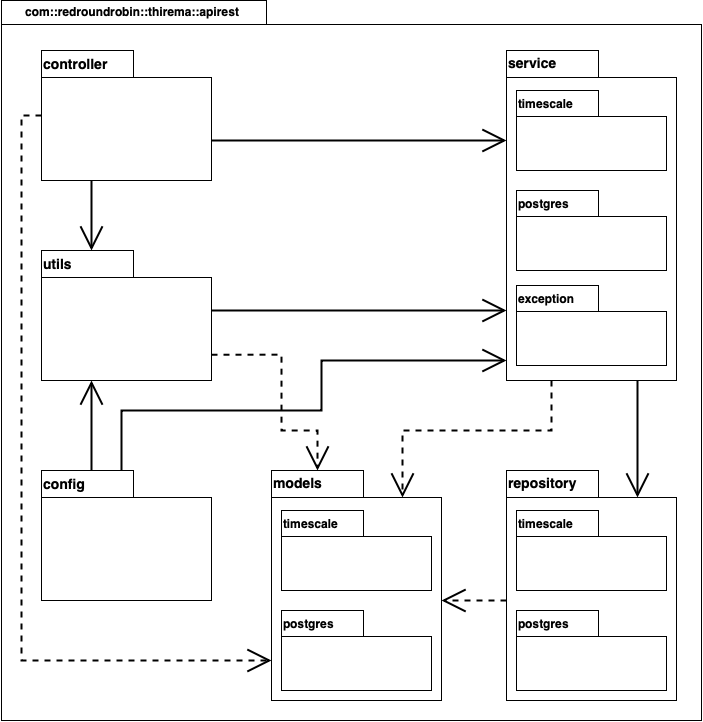
\includegraphics[scale=0.500]{res/images/API/packageAPI.png}
			\caption{Diagramma dei packages per la componente API}
			\label{Diagramma 10}
		\end{figure}

	\subsubsection{Diagrammi delle classi}
		Al fine di semplificare la comprensione delle dipendenze della componente API, si è deciso di suddividere i diagrammi per package, mostrando in dettaglio quelli più significativi.

		
		\begin{figure}[H]
			\centering
			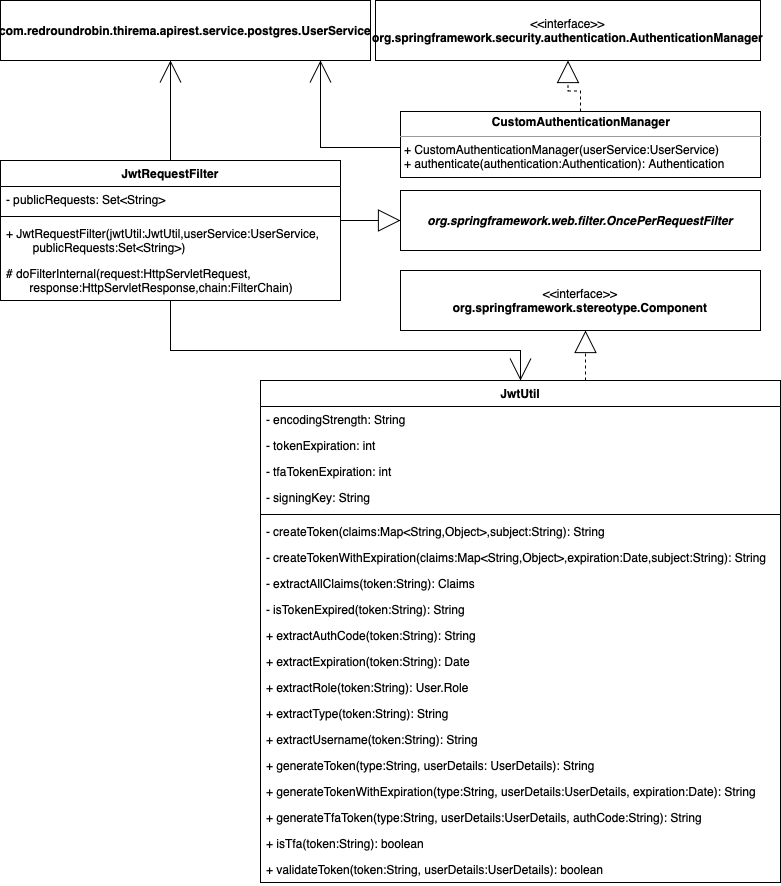
\includegraphics[scale=0.550]{res/images/API/UtilsPackage.png}
			\caption{Diagramma del package utils della componente API}
			\label{Diagramma 11}
		\end{figure}
		\begin{figure}[H]
			\centering
			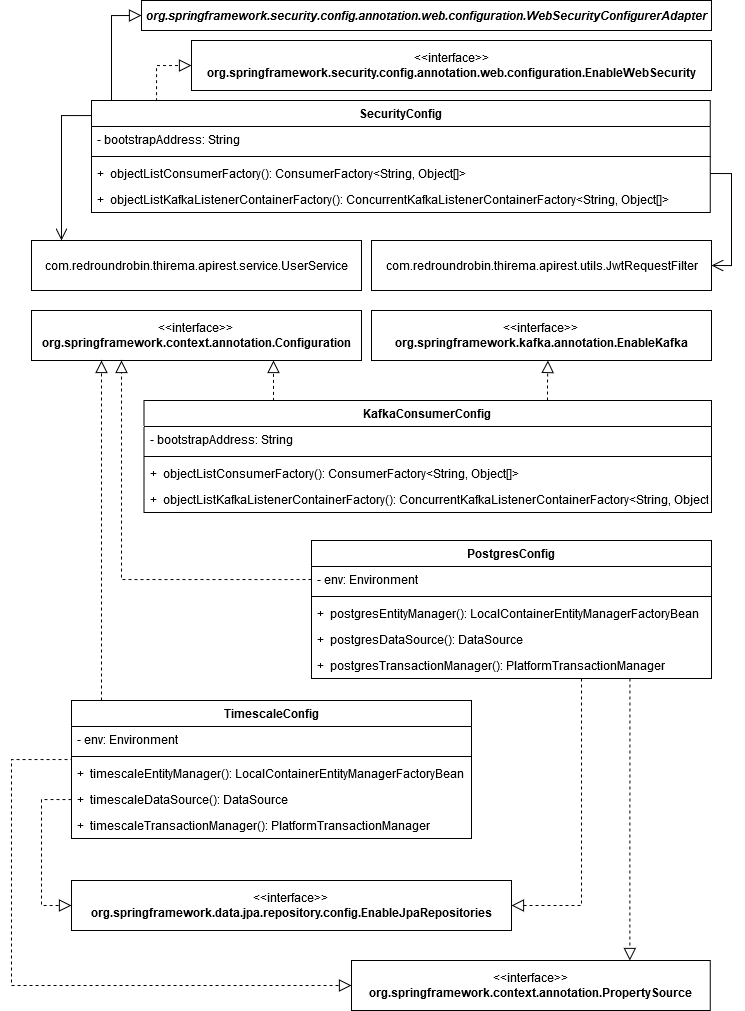
\includegraphics[scale=0.550]{res/images/API/ConfigPackage.png}
			\caption{Diagramma del package config della componente API}
			\label{Diagramma 12}
		\end{figure}
		\begin{figure}[H]
			\centering
			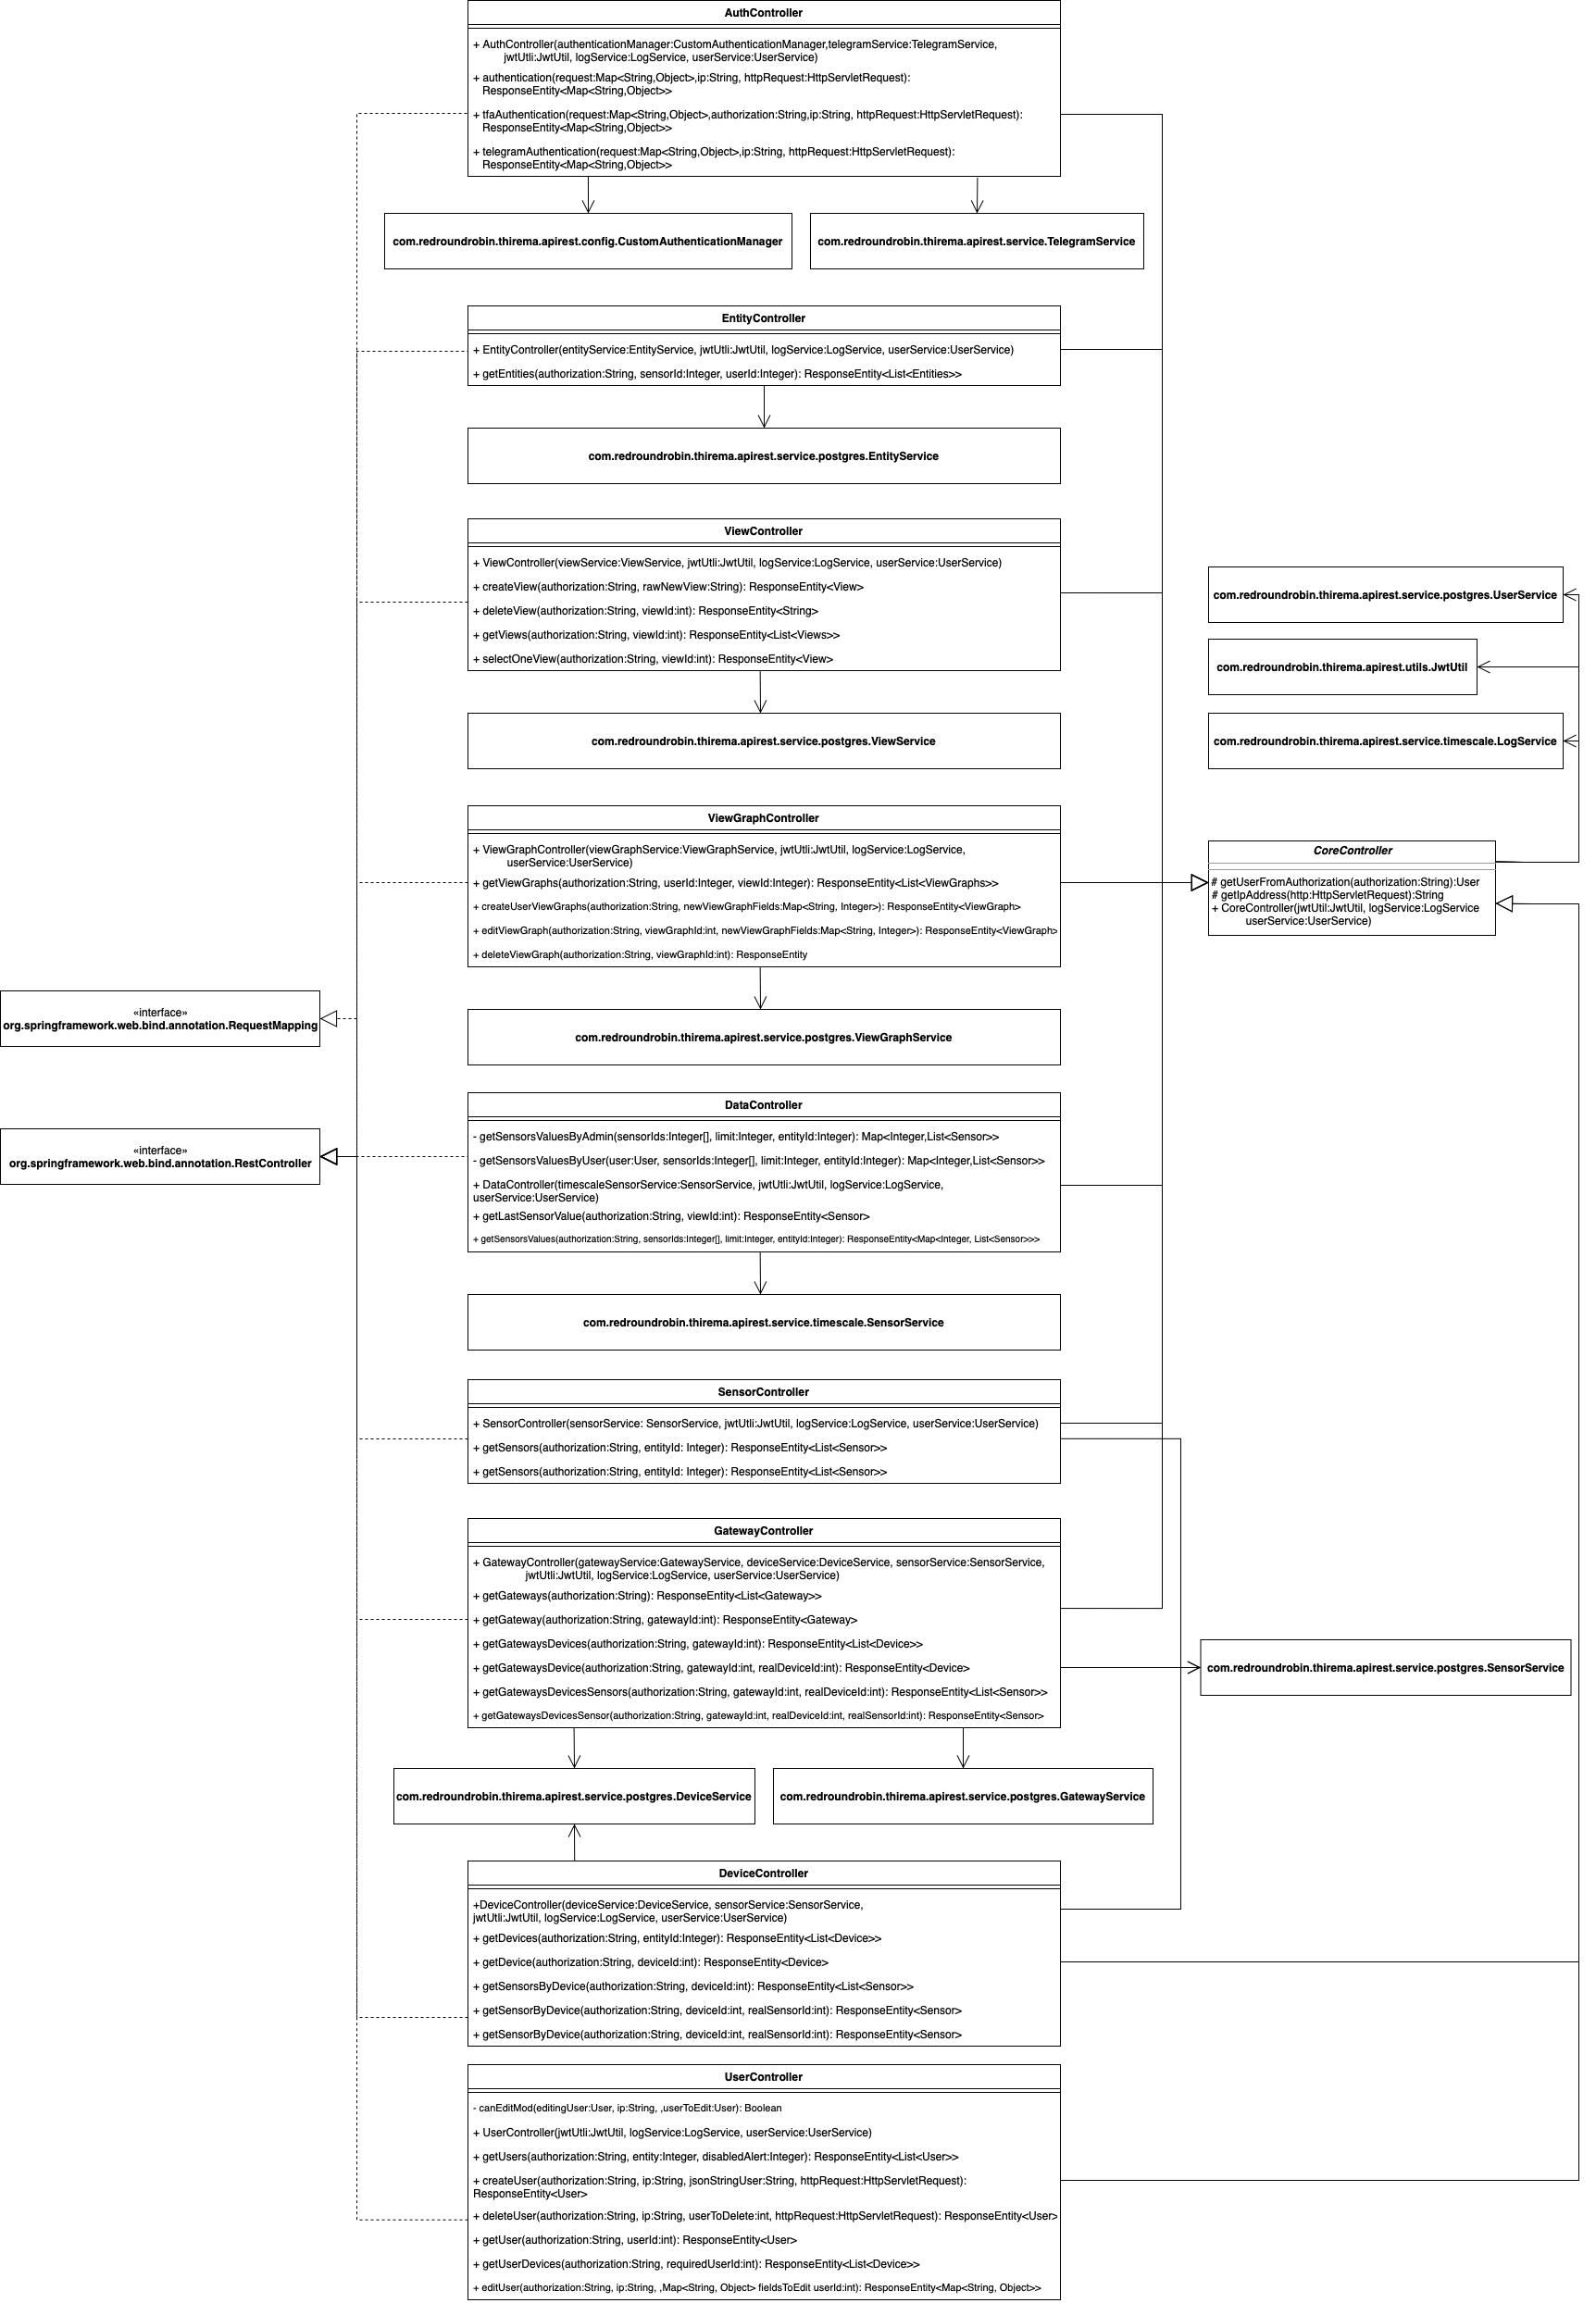
\includegraphics[scale=0.295]{res/images/API/Controllers.png}
			\caption{Diagramma del package controllers della componente API}
			\label{Diagramma 13}
		\end{figure}
		\begin{figure}[H]
			\centering
			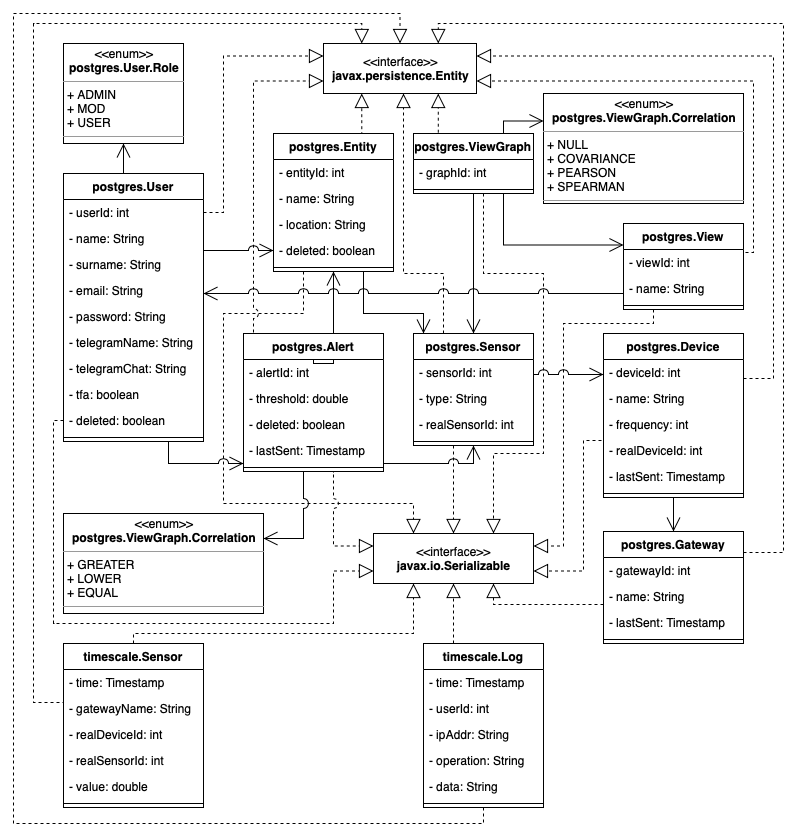
\includegraphics[scale=0.550]{res/images/API/ModelsPackage.png}
			\caption{Diagramma del package models della componente API}
			\label{Diagramma 14}
		\end{figure}
		\begin{landscape}
		\begin{figure}[H]
			\centering
			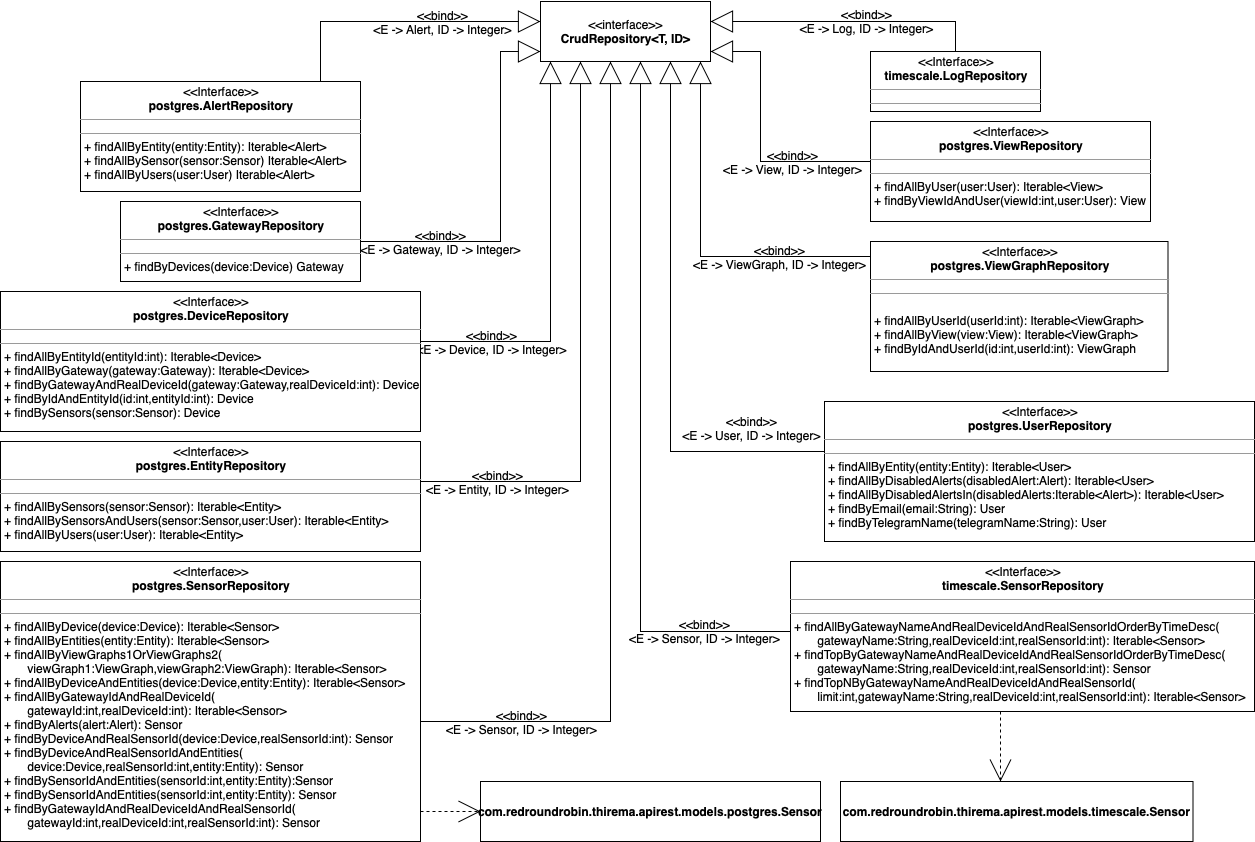
\includegraphics[scale=0.525]{res/images/API/RepositoryPackage.png}
			\caption{Diagramma del package repository della componente API}
			\label{Diagramma 15}
		\end{figure}
		\begin{figure}[H]
			\centering
			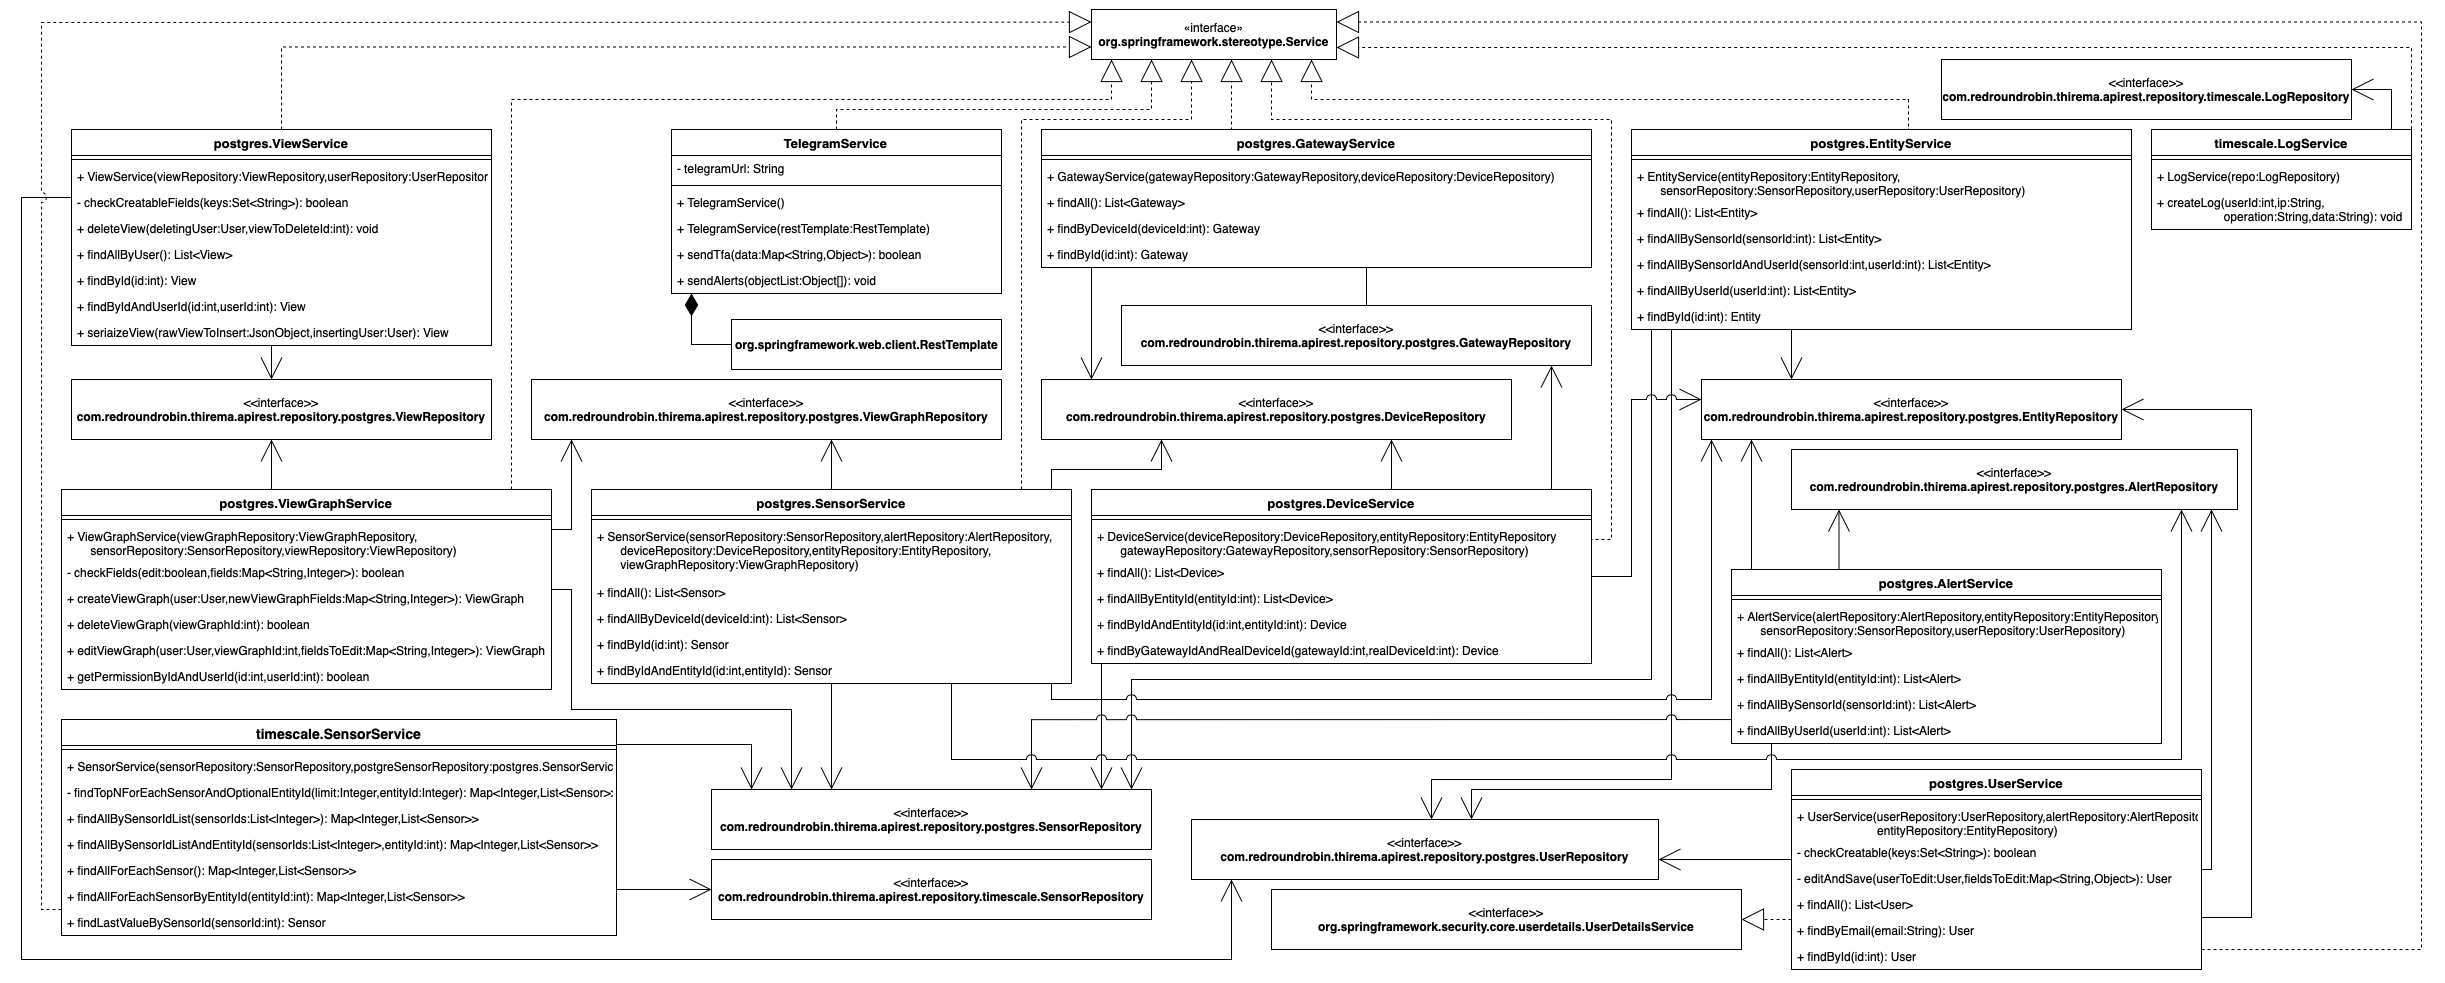
\includegraphics[scale=0.300]{res/images/API/ServicePackage.png}
			\caption{Diagramma del package service della componente API}
			\label{Diagramma 16}
		\end{figure}
		
	\subsubsection{Diagrammi di sequenza}%%%%%%%%%OK
		\begin{figure}[H]
			\centering
			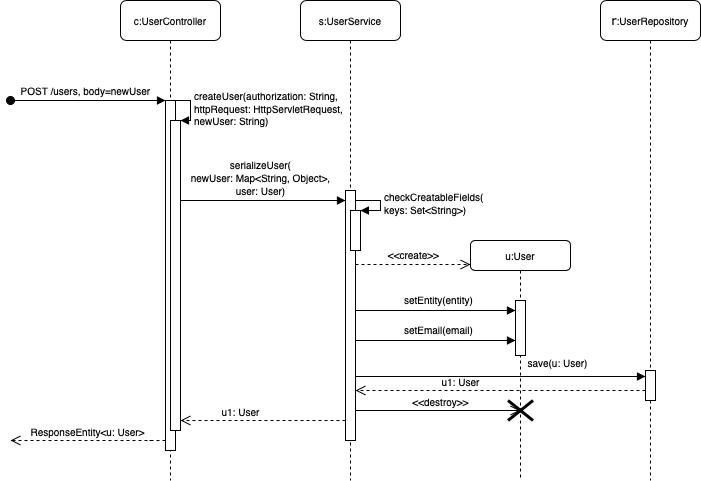
\includegraphics[scale=0.750]{res/images/API/inserimento_utente.png}
			\caption{Diagramma di sequenza che mostra l'inserimento di un utente all'interno della componente API}
			\label{Diagramma 17}
		\end{figure}
		\begin{figure}[H]
			\centering
			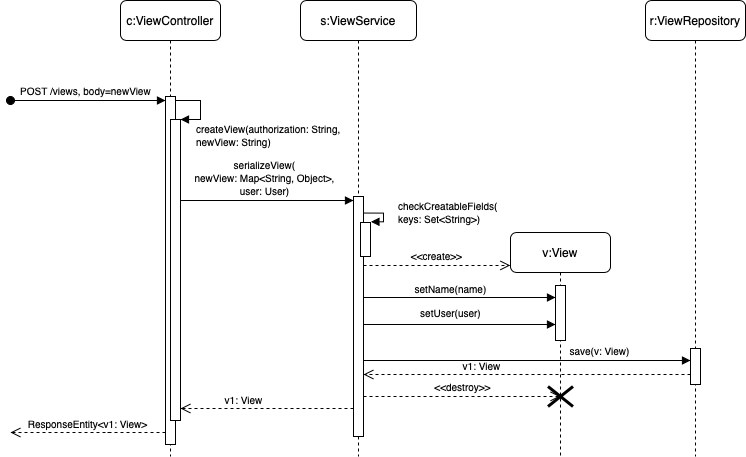
\includegraphics[scale=0.750]{res/images/API/inserimento_view.png}
			\caption{Diagramma di sequenza che mostra l'inserimento di una view all'interno della componente API}
			\label{Diagramma 18}
		\end{figure}
	\end{landscape}